% !TEX TS-program = pdflatex
% !TEX encoding = UTF-8 Unicode

\documentclass[11pt]{article} % use larger type; default would be 10pt


%%% PAGE DIMENSIONS
\usepackage{geometry} % to change the page dimensions
\geometry{a4paper} % or letterpaper (US) or a5paper or\ldots .
% \geometry{margin=2in} % for example, change the margins to 2 inches all round
% \geometry{landscape} % set up the page for landscape
%   read geometry.pdf for detailed page layout information


% \usepackage[parfill]{parskip} % Activate to begin paragraphs with an empty line rather than an indent

%%% PACKAGES
\usepackage{url}
\usepackage{caption}
\usepackage{soulutf8}
\usepackage{booktabs} % for much better looking tables
\usepackage{array} % for better arrays (eg matrices) in maths
\usepackage{paralist} % very flexible & customisable lists (eg. enumerate/itemize, etc.)
\usepackage{verbatim} % adds environment for commenting out blocks of text & for better verbatim
\usepackage{subfig} % make it possible to include more than one captioned figure/table in a single float
% These packages are all incorporated in the memoir class to one degree or another\ldots


%%% HEADERS & FOOTERS
%\usepackage{fancyhdr} % This should be set AFTER setting up the page geometry
%\pagestyle{fancy} % options: empty , plain , fancy




%%My Additional Packages
\usepackage{mathtext}          % русские буквы в формулах
\usepackage[T2A]{fontenc}            % внутренняя кодировка  TeX
\usepackage[utf8]{inputenc}         % кодировка исходного текста
% \usepackage{cmap}          % русский поиск в pdf
%\usepackage[english,russian]{babel} % локализация и переносы
\usepackage[russian,english]{babel} % локализация и переносы

%\usepackage[english]% локализация и переносы

\usepackage{amsmath} % Математические окружения AMS
\usepackage{amsfonts} % Шрифты AMS
\usepackage{amssymb} % Символы AMS
\usepackage{graphicx} % Вставить pdf- или png-файлы

\usepackage{euscript} % Красивый шрифт

\usepackage{longtable}  % Длинные таблицы
\usepackage{multirow} % Слияние строк в таблице

\usepackage[colorinlistoftodos]{todonotes} % [colorinlistoftodos,prependcaption,textsize=tiny]

\usepackage{indentfirst} % Отступ в первом абзаце.
\usepackage{pdflscape} %Переворачивает страницы, удобно для широких таблиц


\usepackage{footnote} %сноски в таблицах
\makesavenoteenv{tabular}
\makesavenoteenv{table}

%\usepackage[backend=biber, style=authoryear, citestyle=authoryear]{biblatex}
\usepackage[backend=biber, style=bwl-FU, citestyle=bwl-FU]{biblatex}
%\usepackage{microtype}

\addbibresource{bibliobase2.bib}

\usepackage{wrapfig} % Обтекание рисунков текстом

\usepackage{hyperref} % Гиперссылки

\DeclareMathOperator{\etr}{etr}
\DeclareMathOperator{\tr}{tr}
\DeclareMathOperator*{\argmax}{arg\,max}
\DeclareMathOperator*{\argmin}{arg\,min}
\DeclareMathOperator{\E}{\mathbb{E}}
\DeclareMathOperator{\diag}{diag}
\DeclareMathOperator{\Var}{\mathbb{V}\mathrm{ar}}
\DeclareMathOperator{\chol}{chol}
\newcommand{\cN}{\mathcal{N}}
\newcommand{\cIW}{\mathcal{IW}}
\newcommand{\lag}{\EuScript{L}}

\newcommand{\prior}{\underline}
\newcommand{\post}{\overline}

\let\vec\relax
\DeclareMathOperator{\vec}{vec}
\hyphenation{re-si-du-als}

%\usepackage[toc,page]{appendix}


%\renewcommand{\appendixtocname}{Приложения}
%\renewcommand{\appendixpagename}{Приложения}
%\renewcommand{\appendixname}{Приложение}
%%% END Article customizations

%%% The "real" document content comes below\ldots

\title{Forecasting Russian macroeconomic indicators with BVAR}
\author{Boris Demeshev and Oxana Malakhovskaya}
\date{} % Activate to display a given date or no date (if empty),
         % otherwise the current date is printed

\begin{document}


\maketitle



\begin{abstract}
 This paper evaluates the forecast performance of Bayesian vector autoregressions on Russian data. We estimate BVAR models  of different size and compare the accuracy of their out-of-sample forecasts with those obtained with unrestricted VARs and RW with drift. We show that many Russian macroeconomic indicators can be forecast by Bayesian VAR more accurately than by competitor models. However, contrary to several other studies, we do not confirm that relative forecast error monotonically decreases with the dimension of the sample. In half of those cases where BVAR appears to be the most accurate model, a small-dimensional BVAR outperforms its high-dimensional counterpart. 
 
 \end{abstract}

\smallskip
\noindent JEL-Classification: C11, C13, C53\\
\smallskip
\noindent Keywords: VAR, forecasting, Bayesian estimation

\section{Introduction}

Accurate macroeconomic forecasts are extremely important for policy making. Time lags are inevitable attributes of any policy, therefore, policy makers should rely on the models with the best possible forecasting performance. Moreover, it is well known that central banks monitor a large set of macroeconomic indicators to determine the policy (\cite{beckner_1996}, \cite{bernanke_boivin_2003}). So a model used for forecasting purposes must be suitable for data-rich samples because large models might outperform the low-dimensional ones by taking into account more potentially relevant information. It explains the recent resurgence of interest of academics, central bankers and private experts for macroeconomic forecasting in data-rich environment.

For the last 30 years, vector autoregressions (VARs) introduced by \cite{sims_1980} have become a  widely-used tool for forecasting. However, it is well known that unrestricted VARs bear the risk of overparametrization even for samples of moderate size. The risk stems from the fact that the number of  parameters to be estimated  increases nonlinearly with the number of equations. For this reason, in economic applications unrestricted VARs usually contain  only up to eight variables and this may potentially lead  to loss of some relevant information and undermine the forecast accuracy. 

As for models in data-rich environment, until recently, several modifications of VARs have been used in empirical studies. They are dynamic factor models (DFM, \cite{forni_al_2000} and \cite{stock_watson_2002})and Panel and Global VARs (PVARs, GVARs, \cite{pesaran_al_2004} and \cite{dees_guntner_2014}).  Dynamic factor models are based on an idea that a relatively small set of indexes extracted from a high-dimensional set of variables can summarize the information from this set.
These factors are treated as variables in a VAR model either separately or in conjunction with several time series from the original information set in a factor-augmented VAR (FAVAR) model. For data sets with panel structure a suitable choice is PVARs and GVARs with shrinkage done by exclusion, exogeneity or homogeneity restrictions.

Another method of shrinkage is the Bayesian one. The shrinkage is done by imposing restrictions on parameters in the form of prior distributions.  While Bayesian VARs (BVARs) in low-dimensional space were widely used for macroeconomic analysis, their use for data-rich environment was limited until 2010. The reason was a general agreement that the Bayesian shrinkage is insufficient to solve the over-parametrization problem in high cross-sectional dimension samples.

However, in their influentual paper,  \cite{demol_al_2008} show that  the Bayesian methods can be successfully applied to a data-rich environment if the degree of shrinkage is set relative to cross-sectional dimension of the sample. \cite{banbura_al_2010} confirm and develop this assertion for BVAR applied to a large set of US time-series. Their main result is that high-dimensional models have better forecasting performance than small-dimensional models and even FAVAR. As a  by-product of the study, they show that accurate forecasts can be already obtained in a medium-size BVAR model (20 variables in their case).

Since 2010, many papers has claimed that, in terms of forecasting accuracy, medium and large BVAR outperform their low-dimensional counterparts. For example,  \cite{beauchemin_zaman_2011} present a medium BVAR with a good forecasting performance applied to the US data.  \cite{bloor_matheson_2010} compare univariate ARs, unrestricted VARs and BVARs and show the evidence that  a high-dimensional BVAR, in general, demonstrates the best forecasting performance in spite of slight deviations for some variables. \cite{koop_2013} claims that  high-dimensional BVARs outperform factor models in terms of forecasting performance. Moreover, he shows that more complicated priors than those that are usually applied may not lead to more precise forecasts. \cite{alessandri_mumtaz_2014} underline the importance of financial factors for an accurate forecast of output and inflation, especially <<for predicting <<tail>> macroeconomic outcomes>>.
\cite{carriero_al_2015} study some characteristics of  BVAR models and find those providing the most accurate forecasts.

The objective of this paper is forecasting of  Russian macroeconomic indicators with BVARs of different size. In spite of the interest that BVARs deserved in international macroeconomic literature, the use of this tool in application to Russian data is extremely scarce. Our underlying hypothesis is that a high-dimensional model can outperform a low-dimensional one in terms of forecasting accuracy. The use of a dynamic factor or a FAVAR model is problematic because of a lack of necessary data. Factor extraction normally  requires at least a hundred time series and, to the best of our knowledge, such a number of relatively long time series for Russian economy does not exist so far. PVARs and GVARs require a panel data structure, so they are more suitable for a multi-country analysis.

Our analysis delivers two important results. First of all, we show that many Russian macroeconomic indicators can be forecasted by Bayesian VAR more accurately than by competitor models. However, contrary to several other studies, we do not confirm that relative forecast error monotonically decreases with the dimension of the sample. In half of those cases where BVAR appears to be the most accurate model, a small-dimensional BVAR outperforms its high-dimensional counterpart. 
 
The paper is structured as follows. Section 2 presents the BVAR methodology and the prior distribution we apply. In Section 3 we describe our sample and data transformation we use. Section 4 contains the results and their interpretation.  Section 5 concludes.


\section{Model}

\subsection{Bayesian VAR}
Let $y_{it}$ be variables stacked in a  $m\times 1$ vector $y_{t}=(y_{1t},y_{2t},\ldots, y_{mt})'$. Reduced form vector autoregression can be written as:
\begin{equation}
y_t =\Phi_{const}+ \Phi_1 y_{t-1} + \Phi_2 y_{t-2} +\ldots + \Phi_p y_{t-p} + \varepsilon_t,\quad \varepsilon_t\sim \cN(0,\Sigma)\label{reduced_var}
\end{equation}
where $\Phi_{const}=(c_1,\ldots ,c_m)'$ --- is a $m\times 1$  vector of constants, $\Phi_l$ --– autoregression   $m\times m$ --- dimensional matrices where $l=1, \ldots, p$. Vector $\varepsilon_t$ --- $m$-dimensional vector of errors with  covariance matrix $\E\varepsilon_t \varepsilon _t'=\Sigma$, and uncorrelated with regressors.
By grouping parameter matrices into one matrix  $\Phi=[\Phi_1 \ldots \Phi_p \; \Phi_{const}]'$ % здесь нужно транспонирование!
and defining new vector $x_t=[ y'_{t-1}\;  \ldots  \; y'_{t-p} \; 1]'$, equation \eqref{reduced_var} can be written in a more compact form:

\begin{equation}
y_t=\Phi' x_t+\varepsilon_t
\end{equation}
If the variables and shocks are grouped in the following way: $Y=[y_1, y_2,\ldots, y_T]'$, $X=[x_1, x_2,\ldots, x_T]'$, $E=[\varepsilon_1, \varepsilon_2,\ldots, \varepsilon_T]'$, the VAR can be written as:
\begin{equation}
Y=X\Phi+E\label{var}
\end{equation}

%We will also use vector $\phi=\vec{\Phi}$ of  $km\times 1$ dimension in what follows.

Bayesian estimate combines a likelihood function $L(Y|\Phi, \Sigma)$ with a prior distribution $p(\Phi, \Sigma)$ and results in a posterior distribution of parameters $p(\Phi, \Sigma|Y)$: %To find the distribution, a corollary from the rule of Bayes is applied:
\begin{equation}
p(\Phi, \Sigma|Y)\propto p(\Phi,\Sigma) L(Y|\Phi,\Sigma)
\end{equation}
%where $ L(Y|\Phi,\Sigma)$ is a likelihood function.


\subsection{Сonjugate Normal-Wishart prior}

Our benchmark model that we use for estimation and forecasting purposes is a Bayesian vector autoregression with a conjugate Normal -- inverted Wishart prior.  The prior can be written as: 

\begin{equation}
\begin{cases} \label{conjugate_prior}
\Sigma\sim \cIW(\prior S, \prior \nu) \\
\Phi|\Sigma\sim \cN (\prior \Phi, \Sigma\otimes\prior \Omega)
\end{cases} 
\end{equation}

The prior mean of coefficients matrices is  written with a $k\times m$ matrix  $\prior \Phi = \E (\Phi)$, where $\prior\Phi=[\prior\Phi_1 \ldots \prior\Phi_p \; \prior\Phi_{const}]'$.% и $\prior \phi = \vec{ \prior \Phi}$. 
The matrices $\prior\Phi_l$ are defined as follows:


\begin{equation}
(\prior\Phi_l)_{ij}=
\begin{cases}
\delta_i\; i=j, l=1;\\
0,\;\text{ otherwise }
\end{cases}\label{minnesota_exp}
\end{equation}

A matrix $\prior \Omega$  is assumed to be diagonal and it depends on several hyperparameters:
\begin{gather}
\prior \Omega=\diag\lbrace{\prior \Omega_{lag=1},\ldots, \prior \Omega_{lag=p},\prior \Omega_{const} \rbrace}\\ 
(\prior \Omega_{lag=l})_{jj} 
=\left(\frac{\lambda}{l^{\lambda_{lag}}\hat\sigma_j}\right)^2
\quad
\prior \Omega_{const}=\lambda_{const}^2 \label{prior_omega2}
\end{gather}

The  hyperparameters have the following interpretation: $\lambda$ determines the overall tightness of the prior and it is responsible for relative weight of the prior with respect to the information incorporated in the data, $\lambda_{lag}$  controls the velocity of decreasing of the prior variance with increasing the lag length, $\lambda_{const}$ governs the relative tightness of the prior for the constant terms.
 
The scale matrix $\prior S$ is diagonal and its nonzero elements assure that the mean of $\Sigma$ is equal to fixed covariance matrix of the standard Minnesota prior: 

\begin{equation}
(\prior S)_{ii}= (\prior \nu- m- 1) \hat\sigma^2_{i}
\end{equation}
The scale parameter $\sigma^2_{i}$ is usually set to be equal to the variance estimate of residuals in a univariate $AR$ model.
The choice of degrees of freedom of inverted Wishart distribution  $\prior\nu$  greater or equal than $\max\lbrace m+2, m+2h-T\rbrace$ guarantees the existence of the parameters prior variance as well as posterior variance of forecasts for horizon $h$ (\cite{kadiyala_karlsson_1997}).

It is possible to show that posterior distribution formed by combining this prior distribution with likelihood function is also Normal --- inverted Wishart (see, for example, \cite{zellner_1996}):
\begin{equation}
\begin{cases}
\Sigma|Y \sim \cIW(\post S, \post \nu) \\
\Phi|\Sigma,Y\sim \cN (\post \Phi, \Sigma\otimes\post \Omega) 
\end{cases}
\end{equation}
with the following parameters:
%где
%\footnote{
%Эквивалентная формула (карлсон p15) для $\post S$, 
%$\post S=\prior S +\hat E'\hat E + (\prior \Phi - \hat \Phi)'(\prior \Omega $+ (X'X)^{-1})^{-1}(\prior \Phi - \hat \Phi)$}
\begin{align*}
\post\nu &=\prior \nu+T\\
\post{\Omega}&=(\prior \Omega^{-1}+X'X)^{-1}\\
\post \Phi&=\post{\Omega}\cdot (\prior \Omega^{-1}\prior \Phi+X'Y)\\
\begin{split}
\post S&=\prior S +\hat E'\hat E+\hat \Phi'
 X'X \hat \Phi \\&+\prior \Phi'\prior\Omega^{-1}\prior \Phi-\post \Phi'\post\Omega^{-1}\post \Phi
 \end{split}\\
\hat\Phi&=(X'X)^{-1}X'Y\\%\quad\text{и }
\hat E&=Y-X\hat\Phi
\end{align*}

There is a popular alternative approach to calculate hyperparameters of the posterior distribution. 
We set $\prior S$ и $\prior \Omega^{-1}$ to be zero matrices and to compensate the difference we add supplementary observations into  $X$ and  $Y$ matrices according to:

\begin{equation}\label{star_sample}
Y^*=\begin{bmatrix}
Y^{NIW} \\
Y 
\end{bmatrix}
\quad
X^*=\begin{bmatrix}
X^{NIW} \\
X 
\end{bmatrix},
\end{equation}
where matrices $Y^{NIW}$ and $X^{NIW}$ are defined as follows\footnote{The similar formulae provided in \cite{banbura_al_2010}, \cite{berg_henzel_2013} can be regarded as special cases of  \eqref{NIW_observations} for $\lambda_{lag}=1$ и $\lambda_{const}\to\infty$.}:
%Можно показать, что подсчет параметров апостериорного распределения  соответствии с указанной схемой эквивалентен добавлению дополнительных искусственных наблюдений по следующей схеме:
%\footnote{The similar formulae provided in \cite{banbura_al_2010}, \cite{berg_henzel_2013} for defining Normal-inverted Wishart distribution can be regarded as special cases of  \eqref{NIW_observations} for $\lambda_{lag}=1$ и $\lambda_{const}\to\infty$.}:

%По аналогии с  работами  \cite{banbura_al_2010}, \cite{berg_henzel_2013} соответствующее априорное распределение вводится путем добавления искусственных наблюдений
\begin{equation}
Y^{NIW}=\begin{bmatrix}
\frac{\diag(\delta_1\sigma_1,\ldots, \delta_m\sigma_m)}{\lambda}\\
0_{m(p-1)\times m}\\
\diag(\sigma_1,\ldots,\sigma_m)\\
0_{1\times m}
\end{bmatrix}
\quad
%
X^{NIW}=\begin{bmatrix}
\frac{\diag(1,2^{\lambda_{lag}},\ldots, p^{\lambda_{lag}})\otimes \diag(\sigma_1,\ldots,\sigma_m)}{\lambda} & 0_{mp\times 1} \\
0_{m\times mp}&0_{m\times 1}\\
0_{1\times mp}&\frac{1}{\lambda_{const}}
\end{bmatrix}\label{NIW_observations}
\end{equation}

This method permits to calculate $\post \Phi$ as an OLS estimate of the regression of $Y^*$ on $X^*$: $\post \Phi=(X^{*\prime}X^*)^{-1} X^{*\prime}Y^*$ and $\post S$ as a sum of squared residuals for this regression: 
$\post S =(Y^* - \post \Phi X^*)'(Y^* - \post \Phi X^*)$.

%При этом математические ожидания и дисперсии априорного распределения параметров могут быть заданы по тому же принципу, что и в априорном распределении Миннесоты (см. \eqref{minnesota_exp}-\eqref{minnesota_variance}).
%При этом априорные распределения параметров, указанные в \eqref{minnesota_exp}-\eqref{minnesota_variance}), предполагают наличие  нулевой априорной корреляции между коэффициентами.


\subsection{Prior modifications}

\cite{doan_al_1984} and \cite{sims_1993} propose to complement this prior distribution with additional information in form of two other priors. The modification expresses a belief that time series may have unit roots and cointegration relations. These elements in the prior allow to avoid unreasonably large share of the variation in the data which is accounted for by deterministic components (\cite{sims_1993}).


A sum-of-coefficients prior was introduced by \cite{doan_al_1984}. If all the time-series in a sample have a unit root, this information can be taken into account with a prior where a sum of all lags parameters for each dependent variable is equal to one (\cite{robertson_tallman_1999}, \cite{blake_mumtaz_2012}). In other words, when a mean of lagged values of a variable is at a certain level, this level is a good forecast for future observations of this dependent variable.  
We implement this prior by combining the dataset given in \ref{star_sample} with artificial dummy-observations according to the following scheme:
%\begin{gather*}
%y_d(i,j)=\begin{cases}
%\post y_{0i}/\lambda_3, \quad \text{если }i=j\\
%0 \quad \text{в обратном случае}
%\end{cases}
%x_d(i,s)=\begin{cases}
%\post y_{0i}/\lambda_3,\quad \text{если }i=j, s<km\\
%0 \quad \text{в обратном случае,}
%\end{cases}
%\end{gather*}
%где $i,j=1,\ldots,m$, $s=1, \ldots, km$. Когда $\lambda_3\to 0$, модель стремится к виду, предполагающему запись в разностях, т.е. единичных корней становится столько же, сколько переменных, и нет коинтеграции.


\begin{gather}
Y^{SC}=\frac{1}{\lambda_{sc}}\begin{bmatrix}\diag(\delta_1\mu_1,\ldots,\delta_m\mu_m)\end{bmatrix}\\
X^{SC}=\frac{1}{\lambda_{sc}}\begin{bmatrix}(1_{1\times p})\otimes \diag(\delta_1\mu_1,\ldots,\delta_m\mu_m) &0_{m\times 1}\end{bmatrix},
\end{gather}

\noindent where $(1_{1\times p})$  is a unitary $[1\times p]$ vector, $\mu_i$ is $i$-th component of vector   $\mu$, that contains the average values of initial observations of all variables in the sample\footnote{Some authors calculate $\mu$  using the average values of all observations in a sample, so that   $\mu=\frac{1}{T}\sum_{t=1}^T y_t$ (\cite{banbura_al_2010} and \cite{carriero_al_2015}). However, following \cite{sims_zha_1998} we calculate $\mu$ using only initial $p$ observations.}: $\mu=\frac{1}{p}\sum_{t=1}^p y_t$.  

The dummy initial observation prior proposed by  \cite{sims_1993} expresses a prior belief that the variables have a common stochastic trend. Only one observation is added so that the values of all variables are equal to an average value of initial observations $\mu_i$ normalized to a scale coefficient $\lambda_{io}$. Therefore, this extra observation is defined as follows:
\begin{gather}
Y^{IO}=\frac{1}{\lambda_{io}}\begin{bmatrix}
\delta_1\mu_1,\ldots,\delta_m\mu_m
\end{bmatrix}\\
X^{IO}=\frac{1}{\lambda_{io}}\begin{bmatrix}
(1_{1\times p})\otimes (\delta_1\mu_1,\ldots,\delta_m\mu_m) &1
\end{bmatrix},
\end{gather}

This prior distribution reflects the belief that an average value for a variable is a linear combination of average values of all other variables.
%%% Непонятно, нужны ли здесть дельты. У Карьеро их нет, но у него и в sum-of-coefficients их нет, а у Банбуры в sum-of-coefficients есть, f initiфд ibservation они не вводят
%\begin{gather*}
%y_d(j)=\begin{cases}\post y_{0i}/\lambda_4 \qquad
%\post y_{0i}/\lambda_4\quad \text{если }s<km\\
%1/\lambda_4 \quad \text{в обратном случае,}
%\end{cases}
%\end{gather*}
%где $j=1,\ldots m, s=1,\ldots km$. 

The hyperparameter $\lambda_{io}$ controls the tightness of this prior. When $\lambda_{io}\to 0 $, the model implies that either all variables are stationary with the mean equal to sample mean of initial observations or nonstationary without drift and cointegrated. 


\subsection{Choice of tightness hyperparameter: the algorithm of shrinkage}

As it is shown by \cite{demol_al_2008} and confirmed in some other recent studies, a sample with a larger cross-sectional dimension requires a lower  $\lambda$, so that the prior must be tighter for a larger sample than for a smaller one. In this paper, we use the approach introduced by \cite{banbura_al_2010} to determine optimal $\lambda$ for every model. 

This algorithm is based on an idea that the shrinkage should be sufficiently tight  to avoid an overparametrization. Moreover, it is assumed that a three-variable unrestricted VAR is parsimonious enough and it does not require any additional shrinkage. It implies that the hyperparameter $\lambda$ may be chosen so that the model has the same in-sample fit as a three-variable VAR.  In other words, any BVAR model is shrinked to the extent of a small unrestricted VAR.  A detailed description of the the procedure is laid out below. Denote  the actual value of a variable $var$ at a moment $T+h$ by $y_{var,T+h}$, and  a forecast of a variable $var$ at a moment $T$ for a  horizon $h$ in a model with $m$ variables and an overall tightness parameter $\lambda$ by  $y_{var,T+h|T}^{\lambda,m}$. The algorithm of choosing $\lambda$ has the following steps. 
\begin{enumerate}
\item We make in-sample one-period forecasts with BVARs on a training sample and calculate mean squared forecast error for set  of $M$ variables of central interest\footnote{Our benchmark set of variables of central interest $(\EuScript{M})$ includes industrial production index, consumer price index and interbank interest rate so that $M=3$. As a step of the robustness check we tried to exclude the interest rate from this set and it didn't almost change the vector of optimal $\lambda$.}:
\begin{equation}
MSFE_{var,1}^{\lambda,m}=\frac{1}{T_0 - p}\sum_{t=p}^{T_0-1} \left(y_{var,t+1|t}^{\lambda,m}-y_{var,t+1}\right)^2,
%\quad var=\lbrace{ip,p,r\rbrace},
\end{equation}
\noindent where  the BVAR coefficients are obtained using the training sample: $t=p+1,\ldots, T_0$ and $T_0$ is the last observation of the training sample: $T_0=p+120$. 
\item In a similar way we calculate one-period forecasts according to random walk (RW) with drift model\footnote{We normalize MSFE for BVAR and VAR models by MSFE obtained with the RW model to take into account the different scales of the series.
We will use a superscript 0 for RW model as RW may be considered as a special case of BVAR if $\lambda=0$ and $\delta_i=1, i=1,\ldots,k$.} for the same variables $\left(MSFE_{var,1}^0\right)$ and a new indicator $FIT^{\lambda,m}$:
% We estimate models for  $m$ variables with many different $\lambda$ and calculate MSF errors  for output  $(MSFE_y^{\lambda,m})$ and prices $(MSFE_{\pi}^{\lambda,m})$  as well as $FIT^{{\lambda,m}}$: 
\begin{equation}
FIT^{\lambda,m}=\frac{1}{M} \sum_{var\in \EuScript{M}} \frac{MSFE_{var,1}^{\lambda,m}}{MSFE_{var,1}^{0}}
%FIT^{\lambda,m}=\frac{1}{2}\cdot\frac{MSFE_y^{\lambda,m}}{MSFE^0_y} + \frac{1}{2}\cdot\frac{MSFE_{\pi}^{\lambda,m}}{MSFE^0_{\pi}}
\end{equation}
\item We estimate  VAR models for the same set of $M$ variables of interest\footnote{We denote all results from unrestricted VAR by a superscript $\infty$ as unrestricted VAR is a special case of BVAR with
$\lambda\to \infty$. In this case the posterior coincides with the likelihood function.} and calculate MSFEs and an indicator $FIT^{\infty,M}$:
\begin{equation}
FIT^{\infty,M}=\frac{1}{M} \sum_{var\in \EuScript{M}} \frac{MSFE_{var,1}^{\infty,M}}{MSFE_{var,1}^{0}}
%FIT^{\infty,M}=\frac{1}{2}\cdot\frac{MSFE_y^{\infty,3}}{MSFE^0_y} + \frac{1}%{2}\cdot\frac{MSFE_{\pi}^{\infty,3},}{MSFE^0_{\pi}}
\end{equation}

\item The optimal lambda is the value minimizing the difference between $FIT^{\lambda,m}$ and $FIT^{\infty,M}$:
\begin{equation}
\lambda^*_m=\argmin_{\lambda} |FIT^{\lambda, m}-FIT^{\infty,M}| 
\end{equation}
\end{enumerate}
After an optimal $\lambda$ is chosen for every $m$, we keep it fixed  and make out-of-sample forecasts on the evaluation sample.  


\subsection{Out-of-sample forecasting}

	We estimate Bayesian VAR models with an optimal  $\lambda$ on <<rolling window>> containing 120 observations, starting from observation $p+2$ and going till March 2015. First $p$ observations are used a pre-sample and the subsample $[p+1, p+120]$ is a training sample used for determining an optimal  $\lambda$ on a grid. We denote the last available observation as  $T_1$, and the last observation of each evaluation subsample as $\tau$. The number of forecasts is equal to $T_1 - T_0 -h +2 $ where $h$ is a forecasting horizon ($h = 1,3,6,9,12)$.  Therefore, the number of one-period forecasts is greater than the number of three-period forecasts by two etc.\footnote{An alternative method is to calculate an equal number of forecasts for each horizon $h$, starting  from $T_0+12$. However it implies a loss of some information about the forecasts and we do not proceed with this method here.}
For every model $m$  and forecasting horizon $h$ we calculate out-of-sample MSFE  for all $m$ variables included in the model:
\begin{equation}
OMSFE_{var,h}^{\lambda,m}=\frac{1}{T_1-T_0-h+1}\sum_{\tau=T_0}^{T_1-h} \\\left(y_{var,\tau+h|\tau}^{\lambda,m}-y_{var,\tau+h}\right)^2,
%\quad var=\lbrace{ip,p,r\rbrace},
\end{equation}
%where $y_{var,T+h}$ - actual values of a variable $var$ at$T+h$,  $y_{var,T+h|T}^{\lambda,m}$ - is a forecast of a variable $var$ at a horizon $h$ in a model with $m$ variables and an overall tightness parameter $\lambda$.

Then we calculate MSFE of out-of-sample forecasts obtained with 
RW $(OMSFE_{var,h}^{0})$ and unrestricted VAR $(OMSFE_{var,h}^{\infty,m})$.
	 
We measure the out-of-sample forecast accuracy in terms of mean squared forecast error: 
\begin{equation}
OMSFE_{var,h}^{\lambda,m}=\frac{1}{2+T_1-T_0-h}\sum_{\tau=T_0-1}^{T_1} (y_{var,\tau+h|\tau}^{\lambda,m}-y_{var,\tau+h|\tau})^2
\end{equation}

To compare the forecast accuracy of different models we report relative MSFE, i.e. the ratio of MSFE of the model in question by the MSFE of a reference model (RW with drift in our case): 

\begin{equation}\label{rmsfe}
RMSFE_{var}=\frac{OMSFE_{var,h}^{\lambda,m}}{OMSFE_{var,h}^0}
\end{equation}
%where $var$ is any variable in the dataset


\section{Data and Estimations}

Our dataset consists  of 23 time series running from January 1996 to April 2015. Our sample containing 232 observations is limited by data availability. The full list of the series and their source is in the Appendix 1. We seasonally adjust data that demonstrate seasonal fluctuations with TRAMO/SEATS option in EViews and apply logarithms to most of the series, with the exception of those already expressed in rates. 

We estimate models of different cross-sectional dimension. Industrial production index, CPI and interbank interest rate are forecast with three-variable, six-variable and 23-variable models.  Monetary aggregate, real effective exchange rate and oil price index are forecast with four-variable, six-variable and 23-variable models. All the other series are forecast  with four-variable, seven-variable and 23-variable models. For all models with dimension less than eight we estimate both unrestricted VAR and BVAR. We estimate only Bayesian VAR on a sample with 23 variables.
The three-variable VAR is the simplest specification that can be justified by a textbook version of a New Keynesian model.  
A model with six variables is specified in line with many monetary models used previously for the structural analysis of different economies (\cite{sims_1992}, \cite{kim_roubini_2000}, \cite{bjornland_2008}, \cite{scholl_uhlig_2008}) and it comprises real effective exchange rate, monetary aggregate M2 and oil price index besides three variables included in the smallest VAR. Oil price index is considered as a variable in the model to reflect a belief that oil price index may be an important explaining factor for the other variables in a sample due to the fact that Russia is an petroleum export-based economy. To forecast variables outside of these core sets we estimate four-variable and seven-variable VARs that contain three or six-variable samples described above plus an additional variable in interest. We include all available time series in our 23-variable model. Totally, after optimal $\lambda$ is chosen, we estimate 79 models. In a compact way the models used for forecasting are presented in the Table \ref{tab:models}. 
Our forecasting horizons are 1, 3, 6, 9 and 12 months and we take all possible lags from 1 to 12. 


\begin{table}
\begin{center}
\caption{List of models and variable sets}
\begin{tabular}{p{2.5cm}l}
\toprule
VAR3/BVAR3&$Y=\lbrace IP, CPI, R \rbrace$\\
VAR4/BVAR4 &$Y=\lbrace IP, CPI, R, Z\rbrace$ \\
VAR6/BVAR6& $Y=\lbrace IP, CPI, R, M2, REER, OPI \rbrace$ \\
VAR7/BVAR7&$Y=\lbrace IP, CPI, R, M2, REER, OPI, W \rbrace$\\
BVAR23&$Y$ includes all 23 variables from the dataset\\
\bottomrule
\end{tabular}
\vspace{5mm}
\caption*{where $IP$ is the industrial production index, $CPI$ is the consumer price index, $R$ is the nominal interbank rate, $M2$ is the monetary aggregate M2, $REER$ is the real effective exchange rate, $OPI$ is the Brent oil price index. $Z$ is any variable from the dataset besides $IP$, $CPI$ and $R$.  $W$ is any variable from the dataset besides $IP$, $CPI$, $R$, $M2$,$REER$, and $OPI$.}
\label{tab:models}
\end{center}
\end{table}

\section{Results}

For every variable and every forecasting horizon we find a model with the lowest RMSFE. We compare 60 specifications for each variable and each forecasting horizon as we have 5 models (VAR and BVAR with 3 or 4 variables, VAR and BVAR with 6 or 7 variables, and BVAR with 23 variables) and 12 lags for each of them. 
We visualize our results with color tables (Figures \ref{fig:rmsfe1}-\ref{fig:rmsfe2} ). 
Two tables in these Figures differ by hyperparameter sets used for BVAR priors. For models depicted in Figure 1  we take $\delta_i =1$ for nonstationary series and $\delta_i =0.5$ for stationary series while constructing the prior. We use KPSS test for splitting the series into two groups. The parameter $\sigma_i$ is taken to be equal standard deviations of residuals in univariate $AR(p)$ model. This hyperparapeter set will be referenced as set A in what follows. Figure 2 is related to BVAR models with prior determined by univariate $AR(1)$ model. We take $\delta_i$ equal to the OLS estimate of the first lag parameter and  $\sigma_i$ equal to standard deviations of residuals in AR(1). This set will be referenced as set B. 


%\begin{figure}
\begin{figure}[!h]
\begin{center}
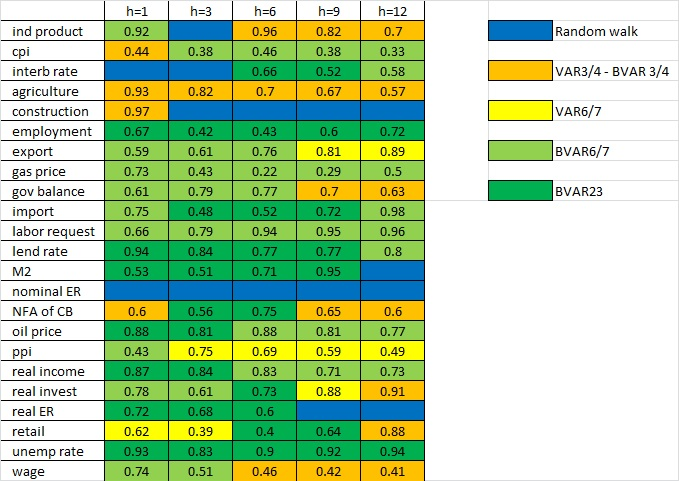
\includegraphics[scale=0.80]{hyper3.jpg}
\caption{RMSFE of the best forecasting accuracy models, parameter set A: $\sigma_i$ are std of $AR(p)$ residuals, $\delta_i=1$ for nonstationary series, $\delta_i=0.5$ for stationary series}
\label{fig:rmsfe1}
\end{center}
\end{figure}



\begin{figure}[!h]
%\begin{figure}
\begin{center}
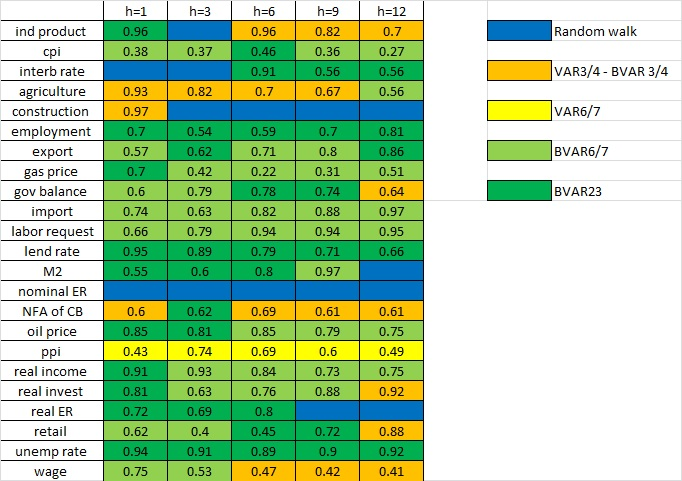
\includegraphics[scale=0.80]{hyper4.jpg}
\caption{RMSFE of the best forecasting accuracy models, parameter set B: $\sigma_i$ are std of $AR(1)$ residuals, $\delta_i=1$ are first lag $AR(1)$ estimates}
\label{fig:rmsfe2}
\end{center}
\end{figure}


A color of a cell corresponds to the model that appears to outperform the others in terms of forecasting accuracy for a given variable and a given forecasting horizon. Most of cells are green (either light green or bright green) reflecting that a BVAR model provides the most accurate forecast for corresponding  variables and forecasting horizons. Unrestricted VAR gives the most accurate forecast for variables and horizons indicated by yellow and orange cells. It is worth to mention that procedure of choosing $\lambda$ is such that BVAR and unrestricted VAR  necessarily coincide  for the smallest sample (3 or 4 variables). It explains why the orange color represents both of these models.  Blue color means that neither BVAR nor VAR can beat random walk in terms of forecast accuracy.

The forecast accuracy is measured with RMSFE calculated according to (\ref{rmsfe}) and is also shown in Figures \ref{fig:rmsfe1}-\ref{fig:rmsfe2}. 
The numbers less than one indicate that a VAR model provides a better forecast than random walk and the smaller the number is, the more accurate the forecasts are relative to random walk.  We see that in most cases we have at least one model that provides a forecast much better than the reference model. 

It is evident that despite different prior parameters sets,  two tables are very similar both in terms of the best forecasting models and  the relative accuracy  with respect to a random walk with drift. 

We can interpret our results in the following way. First of all, for many variables and forecasting horizons of interest, BVAR outperforms random walk and unrestricted VAR. Out of 115 forecasting cases highlighted in the paper (23 variables times 5 forecasting horizons) BVAR appears to be best in terms of forecast accuracy in 71 cases for the prior hyperparameter set A and in 77 cases for the prior hyperparameter set B.  There are variables in our sample that are forecasted more accurately by BVAR for all forecasting horizons of interest  (such as employment, import and lending rate etc). For several variables BVAR is the best option for the shortest horizons (for example, monetary aggregate M2 and real effective exchange rate). To the contrary, for the agricultural production index a BVAR model has the lowest forecast error only on a one-year horizon.  

Secondly, among all cases where BVAR shows its good forecasting accuracy, a high-dimensional BVAR model is the best option roughly in one half cases (35 of 71 for set A and 39 of 77 for set B).  In other cases it is beaten by a low-dimensional BVAR model (6 or 7 variables). 

Thirdly, for some variables and some forecasting horizons neither unrestricted VARs nor BVARs can outperform  the random walk. For example, in all specifications we tried the nominal exchange rate cannot be forecasted by either VARs or BVARs better than RW, and it is a long-lasting consensus in economics remounting to \cite{meese_rogoff_1983}. However, we put into question another wide-spread belief that the price of oil is a random walk process. We show that the oil price index can be forecasted by BVAR much better than by random walk and the result is robust for different prior settings.

\section{Conclusion}

The paper evaluates the forecasting performance of Bayesian vector autoregressions on Russian data. We estimate BVAR models of different size and compare the accuracy of their out-of-sample forecasts with those obtained with unrestricted VARs and RW with drift.   Our sample consists of 23 variables and we forecast at 5 different horizons up to 12 months. We show that for a majority of variables of interest BVAR  outperforms the competing models in terms of forecasting accuracy. 
However, we cannot confirm a conclusion drawn in some other studies where Bayesian methods were applied to data from developed countries. That conclusion claimed that high-dimensional BVARs forecast better than low-dimensional models. Our results implies that a 23-variable BVAR performs most accurately in only about a half of cases where BVAR is considered as a better forecasting tool with respect to its competitors. For the rest of those cases    a BVAR model with a relatively low dimension (6 or 7 variables in our case)   can outperform a 23-variable BVAR in terms of forecasting accuracy.




\newpage

\printbibliography

\newpage

%\begin{appendices}

\section*{Appendices}


\subsection*{Appendix 1. Table of notations}

\begin{center}
\begin{tabular}{ccp{6cm}l}
\toprule
Notation & Dimension &  Description & Formula \\
\midrule
$p$ & scalar & number of lags & \\
$m$ & scalar & number of endogenous variables & \\
$d$ & scalar & number of exogenous variables & \\
$k$ & scalar & number of parameters in an equation & $k=mp+d$ \\
$h$ & scalar & forecast horizon &  \\
\midrule
$y_t$ & $m \times 1$ &  vector of endogenous variables   & $y_t=\Phi' x_t+\varepsilon_t$ \\
$x_t$ & $k \times 1$ & vector of all regressors & $x_t=[ y'_{t-1} \ldots  y'_{t-p} \; z'_t ]'$ \\
$\varepsilon_t$ & $m \times 1$ & vector of random errors & $y_t=\Phi' x_t+\varepsilon_t$\\
$Y$ & $T \times m$ & all endogenous variables & $Y=[y_1, y_2,\ldots, y_T]'$ \\
$X$ & $T \times k$ & matrix of regressors& $X=[x_1, x_2,\ldots, x_T]'$ \\
$E$ & $T \times m$ & matrix of errors & $E=[\varepsilon_1, \varepsilon_2,\ldots, \varepsilon_T]'$ \\
\midrule
$\Phi_1$, \ldots & $m \times m$ & coefficients of VAR & $y_t= \Phi_1 y_{t-1} + \ldots + \Phi_{const} +\varepsilon_t$ \\
$\Phi_{const}$ & $m \times d$ & matrix of constants & $y_t= \Phi_1 y_{t-1} + \ldots + \Phi_{const} +\varepsilon_t$\\
$\Phi$ & $k \times m$ & grouping of matrices $\Phi_1$, \ldots & $\Phi=[ \Phi_1 \ldots \Phi_p \; \Phi_{ex}]'$ \\
\midrule % здесь к независимому без кронекерова произведения
$\prior \Phi$ & $k \times m$ & prior mean $\Phi$ & $\prior \Phi = \E (\Phi)$ \\
$\post \Phi$ & $k \times m$ & posterior mean $\Phi$ & $\post \Phi=\post{\Omega}\cdot (\prior \Omega^{-1}\prior \Phi+X'Y)$\\
$\prior \nu $ & scalar & prior degrees of freedom& $\nu\ge\max\lbrace m+2, m+2h-T\rbrace$ \\
$\post \nu $ & scalar & posterior degrees of freedom & $\post \nu = T + \prior \nu$ \\
$\prior S $ & $m \times m$& prior scale matrix& $\prior S= (\prior \nu- m- 1)\diag(\sigma^2_{1},\ldots,\sigma^2_{m})$\\
$\post S $ & $m \times m$ & posterior scale matrix&  $\post S=\prior S +\hat E'\hat E+\hat \Phi'
 X'X \hat \Phi+$\\&&&$ +\prior \Phi'\prior\Omega^{-1}\prior \Phi-\post \Phi'\post\Omega^{-1}\post \Phi$\\
\midrule % здесь к сопряженному с кронекеровым произведением
$\prior \Omega$ & $k \times k$ & matrix of prior scaling coefficients of covariance matrix $\Phi$& $\prior \Xi = \Sigma \otimes \prior \Omega$ \\
$\post \Omega$ & $k \times k$ & matrix of posterior scaling coefficients of covariance matrix $\Phi$&  $\post \Omega = (\prior\Omega^{-1}+ X'X)^{-1}$,  $\post \Xi = \Sigma \otimes \post \Omega$\\
$\Sigma$ & $m \times m$ &covariance matrix of errors& $\E\varepsilon_t \varepsilon _t'=\Sigma$\\
\bottomrule
\end{tabular}
\end{center}
\newpage
%\begin{landscape}
\subsection*{Appendix 2. Data}
\begin{center}
\begin{table}[h!]
\begin{tabular}{lccr}
\toprule
Name of serie& Type of series &  Base period (if any) & Source \\
\midrule
Industrial production index & base index & 2010 & IFS \\
Consumer price index & base index  & 2010 & IFS \\
Employment in manufacturing index & base index  & 2010 & IFS \\
Interbank interest rate & perc. per ann. &  & IFS \\
Lending interest rate & perc. per ann.&  & IFS \\
Real income index & base index  & 01:1992 & FSSS\\
Unemployment rate & percent &  & IFS \\
Crude oil (Brent) price index & base index  & 2010 & IFS \\
Producer price index & chain index &  & IFS \\
New houses commissioning & thous. of sq. met. &  & FSSS\\
Real fixed investment  index & base index  & 01:1994 & UAESD\\
Real wage rates index & base index  & 01:1993 & FSSS \\
Monetary aggregate М2 & bln. rub.  &  & CBR \\
Real effective exchange rate & base index  & 2010 & IFS \\
Natural gas price & US\$ for bln BTU & 2010 & IFS \\
International reserves excluding gold & Bln US\$ &  & IFS \\
Nominal exchange rate & rub. per US\$. &  & IFS \\
Declared need in workers  & thous. of people &  & UAESD \\
Real agricultural production index & base index  & 01:1993 & UAESD\\
Real retail output index & base index  & 01:1994 & UAESD\\
Total government budgetary balance & bln. rub. &  & UAESD \\
Export of goods & mln US\$ &  & IFS \\
Import of goods &  mln US\$ &  & IFS \\
\bottomrule
\end{tabular}
\vspace{5mm}\\
IFS - International Financial Statistics of IMF \url{http://www.imf.org/en/Data}\\
FSSS - Federal State Statistical Service\url{http://www.gks.ru/}\\
CBR - Central Bank of Russia \url{http://cbr.ru/}\\
UAESD - United Archive of Economic and Sociological Data \url{http://sophist.hse.ru/rstat/}
\end{table}
\end{center}



%\end{landscape}
%\end{appendices}
\end{document} 
